\chapter{书面翻译1}

\title{基于编码树剪枝的HEVC快速编码单元推断方法}

{\heiti 摘要:} 本文为HEVC提出了一种快速决定编码单元划分的方法,这是一种通过基于树剪枝的
策略,来更早推断出编码单元的尺寸的方法。在HEVC中,最为有效的是可变的编码单元尺寸,这是一个
全新的概念。在推断最佳的编码单元尺寸的过程中,作为参考的HEVC编码器会逐个测试每种可能的编码
单元尺寸,以便估测每种情况下,由编码单元尺寸所决定的编码器的表现。在整个编码过程中,这是
主要的计算复杂度来源,因此,为了实现一个高效快速的编码器,这一过程应是攻坚的重点。一种简单的
树剪枝算法是,若当前节点的编码模式已经足够好,那么其子节点的计算均可以被跳过(例如SKIP模式)。
实验结果显示,本文所提出的方法,相较于测试模型3.0下的HEVC编码器,最多有可能达到40 \% 的
时间缩减,而其代价仅仅是一点可以忽略不计的编码效果上的损失。在第六次JCT-VC会议上,本文所提出
的方法被HEVC编码器测试模型4.0所采用。

{\heiti 关键词:} HEVC;编码单元早推断;快速高效视频编码;视频编码。

\section{引言}

2010年,ISO/IEC旗下的组织MEPG和ITU-T旗下的VCEG拟定了一份新的视频编码标准,该标准被称为HEVC。
这份新标准被期望能够满足人们对于视频日益增长的需求,包括压缩效率、视频分辨率、帧率、计算复杂度
等诸多方面。尽管HEVC标准尚处于发展阶段,迄今为止,其压缩效率已经达到了前一标准(MPEG-4 AVC/H.264)
的二倍之高。

虽然HEVC遵循传统的编码结构,包括基于块的运动补偿和变换编码,但实质性改进来自于基于四叉树结构的
新的分层编码概念。在HEVC中,视频编码和解码过程由以下三个单元组成:编码单元(CU),用于作为变换四叉树
的根,以及用于帧间/跳过/帧内预测;预测单元(PU),用于决定模式,包括运动估计和率失真优化;变换
单元(TU),用于变换编码和熵编码。在三种编码单元中,CU对于提升压缩效率是至关重要、最为关键的,
因为它决定了初始编码块的大小,而初始编码块的大小对其他处理单元(例如,PU和TU)的性能影响很大。

当使用CU、PU和TU三种编码单元时,提升压缩效率是可能的,但同时,这也会显着地增加计算的复杂度。通常,
在编码过程中会生成一个四叉树,其中根节点表示最大的CU大小,并且具有对应于下一个CU大小的四个子节点。
这棵树被称为编码树,且其最大深度为4。编码单元与编码树(例如,当根节点的CU大小为64 x 64且树的深度
设定为4的时候,CU0大小为64 x 64,CU1为32 x 32,...,CU3为8 x 8。)被包含在CU尺寸优化的计算与选择中,
这一点导致了CU数量的指数增长(例如,1 x CU0 + 4 x CU1 + 16 x CU2 + 64 x CU3),这一点被直观
地展示在 \ref {fig:trans-cu-demo} 中。由于每一个CU都对应着一个相应的PU和TU的计算,因此,日益
增长的计算复杂对给实时编码器的设计带来了了严峻的挑战。HEVC参考编码器(即,3.0版)大约比MPEG-4 
AVC/H.264参考编码器(即,JM 17.0 高配置版本)慢三倍。为了克服HEVC编码器在计算上的复杂性,我们
提出了基于CU早终止的树剪枝策略,并在JCT-VC第六会议上介绍了该方法。

\begin{figure}[H] % use float package if you want it here
  \centering
  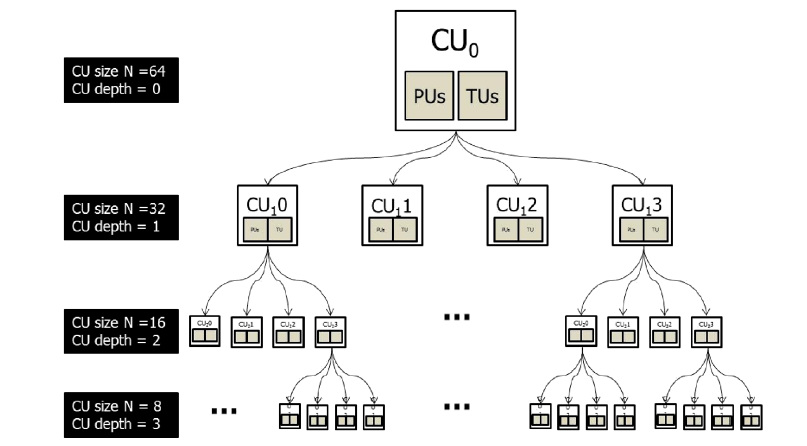
\includegraphics[width = \textwidth]{trans-cu-demo}
  \caption{根节点CU为64 x 64、深度为4的编码树结构示意图}
  \label{fig:trans-cu-demo}
\end{figure}


\section{基于树剪枝的快速编码单元推断}

基于可变CU大小的编码树推断过程计算复杂度可以描述如下:

\begin{equation}
\label{eq-cu-complexity}
\left\{\begin{array}{l}
f(n) = f(n - 1) + 4^n * M_n, f(0) = M_0 \;\; and \\
M_i = {(\frac14)}^i * M_{i - 1}
\end{array}\right.
\end{equation}

这里,$f(n)$ 是当编码树的最大深度被设定为 $n$ 时所需操作的总数,而 $M_i$ 则是
对于第 $i$ 层给定的CU大小所需的操作总数。在 \ref{eq-cu-complexity} 中,我们假定 $M_i$ 是
$M_{i-1}$ 的四分之一是因为CU的大小比起前一层会减少四分之一。总的操作数可以被整合为如下的
公式:

\begin{equation}
\label{eq-cu-complexity-comb}
f(n) = \sum_{i=0}^n 4^i * M_i \cong \mathcal{O} (M_0 * n)
\end{equation}

如 \ref{eq-cu-complexity-comb} 所展示,计算的复杂度随着CU深度的增加单调增加。当考虑到 $M_i$
代表着包括对每个CU大小的运动估计在内的整个编码过程这一事实,最大CU深度就自然成为了决定编码时间
的主要因素。

本文研究了一种通过更早地确定CU的深度来加速CU深度推断的策略。我们利用了这样一个事实,当当前CU节点
的代价低于该节点子节点的代价时,我们就不必再对子树进行进一步的处理(例如,$RDCost(CU_t) < \sum_{i=0}^3 RDCost(CU^i_{t-1})$)。
这一方法的唯一问题是,子树的代价必须是已知的,这一要求妨碍了子树计算复杂度的减少程度。我们可以避免
子树代价的计算,如果当前节点的代价已经是最小的了(例如,SKIP模式),而这正是本方法的核心概念。
为了进一步减少计算复杂度,我们可以定义剪枝的条件如下:

\begin{equation}
\label{eq-pruning-condition}
\begin{split}
Pruning & \; codition: \\
(\mathop{m'} & =  \mathop{argmin}\limits_{m \in Mode} RDCost(CU_t | PU=m)) \le Threshold \\
Mode & = \{ SKIP, Inter2Nx2N, Inter2NxN, InterNx2N, InterNxN \} 
\end{split}
\end{equation}

这里,Mode表示按根据复杂度确定的预测模式的有序集合,而 $\mathop{m'}$ 则是为当前CU深度选择的
预测模式,且Threshold将根据Mode选择。在 \ref{eq-pruning-condition} 中,通过从SKIP到InterNxN,不断
改变Threshold的值,剪枝过程的可能性将被推断。若Threshold被设置为SKIP时,剪枝过程将不会对压缩效率产生
影响;否则,以降低压缩效率为代价,更多的子树将被剪去。根据上述分析,我们提出了 \ref{trans-algorithm} 
所示的剪枝过程。


\begin{figure}[H] % use float package if you want it here
  \centering
  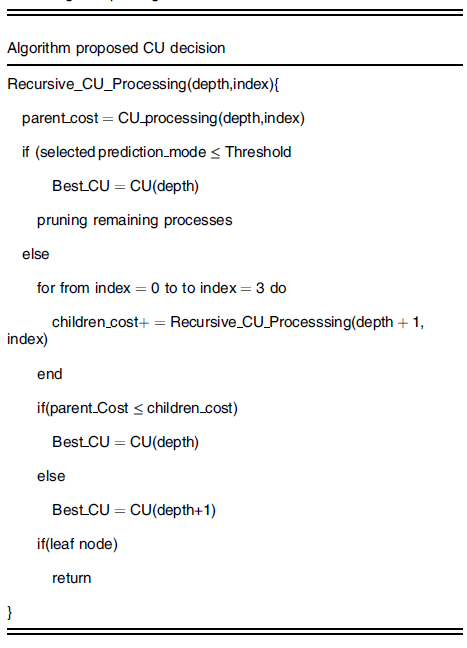
\includegraphics[width = 0.6\textwidth]{trans-algorithm}
  \caption{基于树剪枝的CU推断方法的步骤}
  \label{fig:trans-algorithm}
\end{figure}

\section{实验结果}

为了进行性能评测,我们测试了了我们的方法与HM 3.0两种方法的总执行时间,以确认计算复杂度的降低
程度。编码的表现以 $\Delta Bitrate[ (B_{PRO} - B_{REF})/B_{REF} X 100 ]$ 和 
$ \Delta PSNR(P_{PRO} - P_{REF})$ 来衡量,并且时间的减少以 $ \Delta Time[ (T_{PRO} - T_{REF})/T_{REF} X 100 ]$
来衡量。在实验中,我们吧Threshold值设置为SKIP模式。有关编码环境的更多细节在 \ref{fig:trans-cfg} 被展示。

\begin{figure}[H] % use float package if you want it here
  \centering
  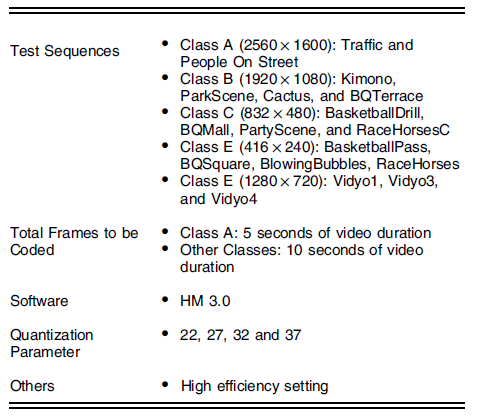
\includegraphics[width = 0.6\textwidth]{trans-cfg}
  \caption{测试环境与软件参考配置}
  \label{fig:trans-cfg}
\end{figure}

\begin{figure}[H] % use float package if you want it here
  \centering
  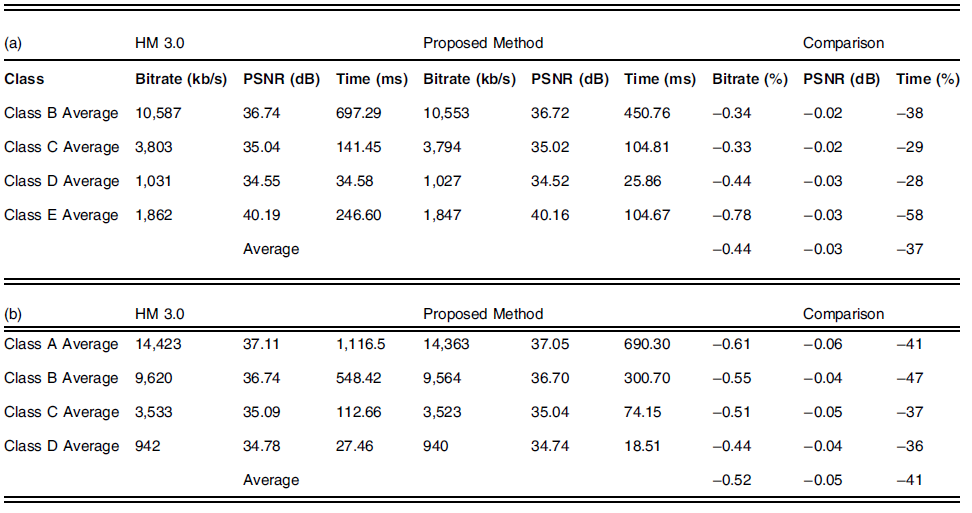
\includegraphics[width = \textwidth]{trans-result}
  \caption{文中所提出的算法与HM3.0在编码时间上的对比:(a)低延迟方案;(b)随机访问方案}
  \label{fig:trans-result}
\end{figure}

\ref{fig:trans-result} 展示了在低延迟方案与随机访问方案两种环境下,我们评测了我们的方法与
HM 3.0两种方法的总执行时间。尽管我们测试了每一种 \ref{fig:trans-cfg} 中所列举的不同的量化参数下的结果,
但 \ref{fig:trans-result} 中,我们只展示每一类的平均结果。 \ref{fig:trans-result} 显示了我们的
方法相较于HM 3.0,,在低延迟方案的环境下减少了63.34\%的时间,而在随机访问方案的环境下,则减少了
59.43 \%的时间。以图像质量的轻微退化为代价所获得的编码增益,是所提出的方法的自然结果,因为编码树修剪过程
会使图像质量上的比特减少。通过调整Threshold的值,我们可以节约更多的编码时间,但其代价是图片质量
的进一步下降。目前,我们所提出的方法,在模式设置为SKIP时,能得到编码时间与图片质量相平衡的最好结果。


\section{结论}

在本文中,我们为HEVC提出了一种快速的CU决策方法,这种方法基于编码树修剪从而更早确定CU的大小,与HM 3.0
编码器相比,仅以可以忽略不计的BD-比特率损失为代价,就可以使编码时间减少约40 \%。实验结果表明,当你想设计
一个快速的HEVC编码器时,我们所提出的编码树剪枝方法应当被考虑。在JCT-VC第六次会议上,HEVC测试模型4.0
编码器采用了我们所提出的方法。


\chapter{书面翻译2}

\title{一种有效的H.264上的可变块大小早终止算法}

{\heiti 摘要:} H.264视频编码标准比以前的标准提供了更高的编码效率,但同时,其复杂度也显著提高。
在H.264编码器中,最耗时的组成部分是可变块大小的运动估计。为了降低运动估计的复杂度,本文提出了一种
早终止算法。它通过检查仅仅一个搜索点来预测最佳的运动矢量。使用该方法,一些运动搜索可以被提前停止,
由此,大量的搜索点可以被跳过。本文所提出的方法适用于任何快速运动估计算法。实验采用的是H.264所采用的
一种快速运动估计算法。结果表明,本算法显著降低了复杂度,而代价仅仅是可以忽略不计的视频质量的降低。

{\heiti 关键词:} 早终止;H.264;运动估计;可变块大小。

\section{引言}

近年来,视频编码技术高速发展。理所当然地,压缩性能的提升伴随着计算代价的增长。作为ITU-T的VCEG和
ISO/IEC的MPEG所最新制定标准的H.264,相较于之前的H.261、H.263、MPEG-1/2/4等标准,在编码效率上有着
巨幅的提升。然而,其过高的计算复杂度使其无法被广泛应用到实时业务中。

通常来说,一个视频编码器最为耗时的部分是运动估计。减少其计算代价的方法有两种。第一种是加速算法本身,
对ME过程来说,数种快速算法被提出,例如六边形搜索(HBS)、增强型预测分区搜索(EPZS)和混合非对称
交叉多六边形网格搜索(UMHexagonS)等。另一种方法就是更早地终止ME的计算。通过预测那些DCT系数会被量化
为0的块,一些方法有效地减少了ME的计算量。另一方面,一些块的重要部分在ME之后具有零运动矢量(MV)。
据此,有算法提出的零运动检测算法(ZMD),通过将它们的差值的绝对值求和,并与预先定义的阈值进行比较来检测这样的块,
然后跳过其余的搜索点。

然而,上述早终止方法都是针对以前的编码方案(如H.263)而开发的。它们不能再应用于H.264。这是因为相比于仅有
两中块大小(16x16和8x8)的H.263,H.264拥有从16x16到4x4变化的七种块大小。

通过扩展ZMD的概念,我们提出了一种用于H.264视频编码的可变块大小最佳运动检测(VBBMD)算法。
该方法在三个方面与ZMD不同:

\begin{enumerate}
  \item 基于不同块大小的检测精度,分别获得VBBMD中使用的阈值,同时考虑了复杂度的降低,使得阈值的决策更加合理;
  \item 在VBBMD中,除零运动点外,预测的移动到的点也会被检查,从而更多的搜索点可以被跳过;
  \item 对于16x16的块,VBBMD使用双阈值。使用较低的阈值跳过较小的块的运动搜索。
\end{enumerate}

我们的方法可以适用于任何运动搜索算法,并且不需要额外的计算。注意,整个讨论集中于帧间帧(P帧)和
整数像素运动搜索。文章的剩余部分如下进行组织。 \ref{sec:app2-early-termination} 介绍了早期终止算法
及其改进。 \ref{sec:app2-sim-result} 中给出了仿真结果。最后,在 \ref{sec:app2-conclusion} ,
我们总结了本文,并给出了未来的方向。

\section{早终止算法}
\label{sec:app2-early-termination}

\subsection{可变块大小零运动推断}

\subsection{可变块大小最佳运动推断}

\section{模拟结果}
\label{sec:app2-sim-result}


\section{结论}
\label{sec:app2-conclusion}


本文提出了一种H.264视频编码的早终止方法VBBMD,该方法通过进一步减少计算总量来帮助现有的快速运动搜索
算法。该方法通过检查一个搜索点来预测最佳的MV。通过这种方法,一些运动搜索可以被提前停止,因此与这些
搜索相关联的计算可以被减少。在该方法中,考虑了复杂度的降低的同时,阈值通过基于不同块大小的检测精度来确定,
这使得阈值决策更加合理。实验结果表明,我们提出的方法实现了显著的复杂度降低,而视频质量的退化是可以忽略不计的。
未来的方向可能包括使阈值根据量化级别和运动级别自适应调整,并将早终止方法应用于子像素的运动估计。
